% !TEX root =  ../main_manuscript.tex 
\section{Simulation Study}
\label{sec:sim_study}
Although we evaluated personalized schedules for a demonstration patient, we also intend to analyze and compare personalized and fixed schedules in a full cohort. Our criteria for comparison of schedules are the total number of invasive tests planned (burden), and the actual time delay in detecting progression (shorter is beneficial) for each schedule. Due to the periodical nature of schedules, the actual time delay in detecting progression cannot be observed in real-world surveillance. Hence, instead, we compare personalized versus fixed schedules via an extensive simulated randomized clinical trial in which each hypothetical patient undergoes each schedule. To keep our simulation study realistic, we employ the prostate cancer active surveillance scenario. Specifically, our simulated population is generated using the joint model fitted to the PRIAS cohort (Supplementary~B).

\subsection{Simulation Setup}
From the simulation population, we first sample 500 datasets, each representing a hypothetical prostate cancer surveillance program with 1000 patients in it. We generate a true cancer progression time for each of the ${\mbox{500} \times \mbox{1000}}$ patients, and then sample longitudinal DRE and PSA measurements biannually (PRIAS protocol) for them. We split each dataset into training (750 patients) and test (250 patients) parts, and generate a random and non-informative censoring time for the training patients. All training and test patients also observe Type-I censoring at year ten of follow-up (current study period of PRIAS). We next fit a joint model of the same specification as the model fitted to PRIAS (Supplementary~B), to each of the 500 training datasets and retrieve MCMC samples from the 500 sets of the posterior distribution of the parameters. In each of the 500 hypothetical surveillance programs, we utilize the corresponding fitted joint models to obtain the cumulative-risk of progression in each of the ${\mbox{500} \times \mbox{250}}$ test patients. These cumulative-risk profiles are further used to create personalized biopsy schedules for the test patients. 

For each test patient, we conduct hypothetical biopsies using two fixed (PRIAS and annual schedule) and three personalized biopsy schedules. Personalized schedules are based on, a fixed risk threshold $\kappa=10\%$, an optimal current visit time $v$ specific threshold $\kappa^*(v)$ chosen via~(\ref{eq:kappa_choice}), and an optimal threshold obtained under the constraint that expected time delay in detecting progression is less than 0.75 years (9 months), denoted $\kappa^*\{v \mid E(\mathcal{D})\leq 0.75\}$. The choice of 0.75 years delay constraint is arbitrary and is only used to illustrate that applying the constraint limits the average delay at 0.75 years. Successive personalized biopsy decisions are made only on the standard PSA follow-up visits, utilizing clinical data accumulated only until the corresponding current visit time~(\ref{eq:personalized_decision_grid}). We maintain a minimum recommended gap of one year between consecutive prostate biopsies~\citep{bokhorst2015compliance} as well. Biopsies are conducted until progression is detected, or the maximum follow-up period at year ten (horizon) is reached. The actual time delay in detecting progression is equal to the difference in time at which progression is detected and the actual (simulated) time of progression of a patient.

\subsection{Simulation Results}
In the simulation study, nearly 50\% of the patients observed progression during the ten year study period (\emph{progressing}) and 50\% did not (\emph{non-progressing}). While we can calculate the total number of biopsies scheduled in all $500 \times 250$ test patients, the actual time delay in detecting progression is available only for progressing patients. Hence, we show the simulation results separately for progressing and non-progressing patients (Figure~\ref{fig:simulation_boxplot}).

Before discussing delay in detecting progression (Panel~A, Figure~\ref{fig:simulation_boxplot}), we note that mean delay up to 1.7 years in all patients~\citep{inoue2018comparative}, and up to three years in patients who progress after year one of follow-up~\citep{carvalho}, may not increase risks of adverse outcomes later. In this regard, the annual biopsies guarantee a maximum delay of one year in all patients. However, they also schedule the highest number of biopsies (Median~3, Inter-quartile range or IQR:~1--6). Much fewer biopsies are planned by the PRIAS schedule (Median~2, IQR:~1--4), but it also has a higher time delay (Median~0.74, IQR: 0.38--1.00 years). The personalized schedule based on optimal risk threshold $\kappa^*(v)$ schedules fewer biopsies than PRIAS and has a delay~(Median~0.86, IQR:~0.46--1.26 years) slightly higher than PRIAS. The expected delay for risk threshold optimized with a constraint on expected delay $\kappa^*\{v \mid E(D)\leq 0.75\}$ is equal to 0.61 years, i.e., the constraint works as expected.

The simulated non-progressing patients (Panel~B,~Figure~\ref{fig:simulation_boxplot}) gained the most with personalized schedules. The annual schedule plans 10 (unnecessary) biopsies for each such patient, and the PRIAS schedule plans a median of 6~(IQR:~4--8) biopsies. In contrast, the personalized schedule based on optimized risk threshold $\kappa^*(v)$ plans fewer biopsies consistently (Median~6, IQR:~6--7). The 10\% threshold based schedule plans even fewer biopsies (Median~5, IQR:~4--6).

\begin{figure}
\centerline{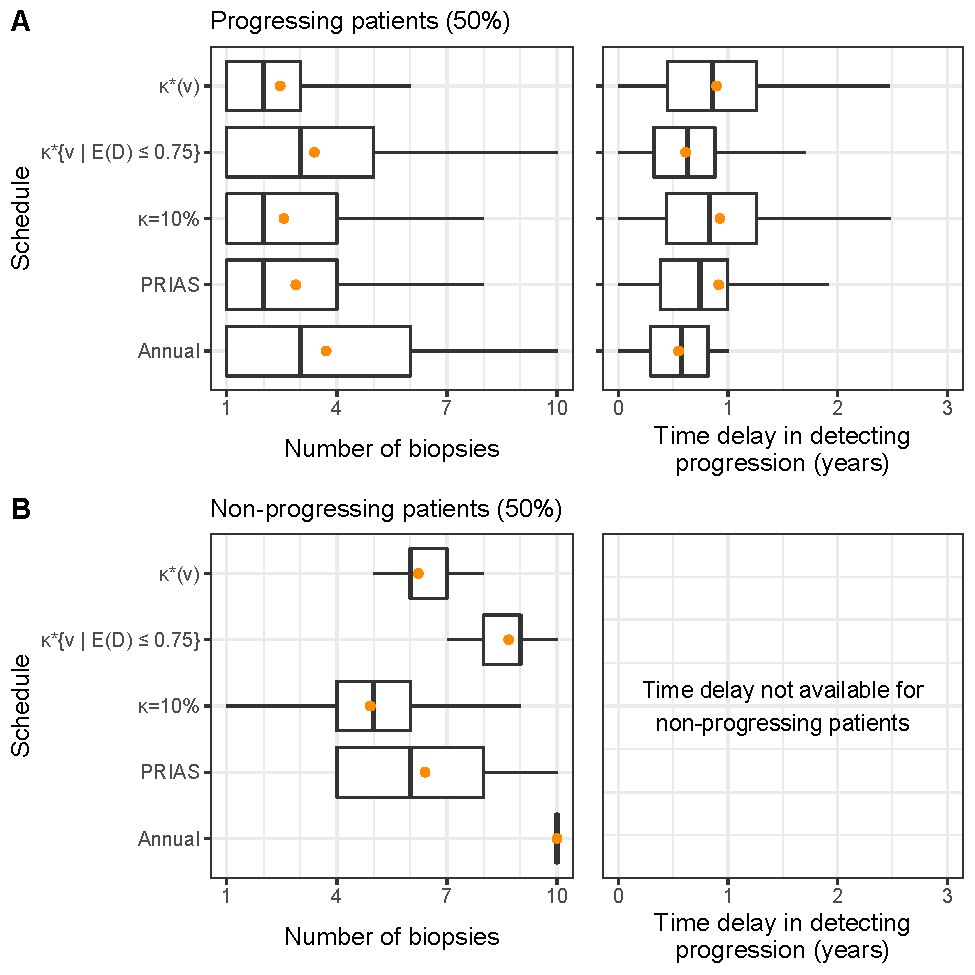
\includegraphics{images/simulation_boxplot.pdf}}
\caption{\small{\textbf{Number of biopsies and the time delay in detecting cancer progression for various biopsy schedules} obtained via a simulation study. \textbf{Mean} is indicated by the orange circle. Time delay (years) is calculated as (time of positive biopsy - the actual simulated time of cancer progression). Biopsies are conducted until cancer progression is detected. \textbf{Panel~A:} simulated patients who obtained cancer progression in the ten year study period (progressing). \textbf{Panel~B:} simulated patients who did not obtain cancer progression in the ten year study period (non-progressing). Types of schedules: ${\kappa=10\%}$ and $\kappa^*(v)$ schedule a biopsy if the cumulative-risk of cancer progression at the current visit time $v$ is more than 10\%, and an automatically chosen threshold~(\ref{eq:kappa_choice}), respectively. Schedule ${\kappa^*\{v \mid E(\mathcal{D})\leq 0.75\}}$ is similar to $\kappa^*(v)$ except that the euclidean distance in~(\ref{eq:kappa_choice}) is minimized under the constraint that expected delay in detecting progression is at most 9 months (0.75 years). Annual corresponds to a schedule of yearly biopsies, and PRIAS corresponds to biopsies as per PRIAS protocol (Section~\ref{sec:results}).}}
\label{fig:simulation_boxplot}
\end{figure}